\documentclass[12pt,twoside]{scrreprt}
\usepackage[T1]{fontenc}
\usepackage[utf8]{inputenc}
\usepackage{lmodern}
\usepackage{textcomp}
\usepackage[francais]{babel, varioref}
\usepackage{graphicx}
\usepackage{listings}
\usepackage{xspace}
\usepackage{amsmath}
\usepackage{amssymb}
\usepackage{enumitem}
\usepackage{calc}
\usepackage{listingsutf8}
\usepackage{color}
\usepackage{xcolor}
\usepackage{afterpage}
\usepackage[style=verbose-note,backend=bibtex]{biblatex}
\usepackage{url}
\usepackage[top=2.1cm,bottom=2.2cm,left=2cm,right=2cm]{geometry}
\usepackage[final]{pdfpages}
\usepackage{subcaption}
\usepackage{amsmath}
\usepackage{array}
\usepackage{mathrsfs}
\frenchbsetup{StandardLists=true}
\captionsetup{compatibility=false}

\newcommand{\hlc}[2][yellow]{ {\sethlcolor{#1} \hl{#2}} }
\newcommand{\highlight}[2][yellow]{\mathchoice%
  {\colorbox{#1}{$\displaystyle#2$}}%
  {\colorbox{#1}{$\textstyle#2$}}%
  {\colorbox{#1}{$\scriptstyle#2$}}%
  {\colorbox{#1}{$\scriptscriptstyle#2$}}}

\definecolor{gray}{rgb}{0.4,0.4,0.4}
\definecolor{darkblue}{rgb}{0.0,0.0,0.6}
\definecolor{cyan}{rgb}{0.0,0.6,0.6}

% Pour sommaire cliquable
\usepackage{hyperref} % Créer des liens et des signets
\hypersetup{
colorlinks=true, %colorise les liens
breaklinks=true, %permet le retour à la ligne dans les liens trop longs
urlcolor= blue, %couleur des hyperliens
linkcolor= black, %couleur des liens internes
citecolor=black,  %couleur des références
}

% Fichier de bibliographie
\bibliography{parties/biblio}

\usepackage{templateINSA}
\initINSA

% Tirte centre
\renewcommand\infoBig{Baptiste O'Jeanson}
\renewcommand\infoSmall{Report of Machine Learning Project}

% Titre bas
\title{Competitive Machine learning}
\renewcommand\soustitre{Classifying Default Application for Peer-to-Peer Bitcoin Loans}

% Auteurs
\author{\textbf{Student:} Baptiste \bsc{O'Jeanson} \\
	\textbf{Teacher:} Tobias \bsc{Scheffer}\\
	\textbf{Year:} 2015-2016\\
	\textbf{Place:} Potsdam University\\}

\begin{document}

% titleINSA : Page de garde
% #1 : descendre le titre du milieu (en mm)
% #2 : lien de l'image de fond
% #3 : décalage sur X de l'image de fond (en mm)
% #4 : décalage sur Y de l'image de fond (en mm)
% #5 : largeur de l'image de fond de #5 (en mm)
% #6 : Crédit de l'image de fond
 \titleINSA{0}{images/uni_potsdam.png}{0}{100}{220}{}

% Sommaire
\tableofcontents

% Parties
\chapter{Introduction}
The evolution of technologies transformed a lot of ways of doing usual business. And the banking sector did not miss this transformation. In fact, with some major banking crisis people created some new way of trading money and the Bitcoin currency was born.\\

Bitbond is a startup offering to everyone the possibility to borrow money in affordable terms or to lend money with profitable interest rate. Bitbond operates thanks to a peer-to-peer Bitcoin lending platform. Thanks to their idea, small businesses get access to affordable loans while lenders earn profitable interest rates. Since Bitbond works exclusively with the digital currency Bitcoin, neither the borrower nor the lender need a bank account to participate in our global loan market. Bitbond's mission is to make investing and financing globally accessible.\\

The main purpose of this project is to use the data of Bitbond (which are accessible to everyone) to analyse it and follow a machine learning procedure to identify the financial risks.\\

Anyone who wish to get a loan must satisfy some requirements :
\begin{enumerate}
    \item He must register on the platform ;
    \item He must inform about his name, his gender, his date of birth and his country of citizenship ;
    \item He must inform about his phone, his address and if he had moved within the last 3 months ;
    \item He must inform about his employment (self-employed, salaried, retired, etc.) ;
    \item He must inform about different account he may have (ebay, paypal, facebook, etc.) to show his healthy activity ;
\end{enumerate}
Then, Bitbond uses all those informations to compute indicators. In fact, those informations allow Bitbond to assess the ability of the borrower to pay back a loan : the creditworthiness (represents by a letter).\\

To get this indicator, Bitbond asks for credit informations and compute a score. This score conducts the rating for the creditworthiness, as well as the type of employment, the connection of the personal PayPal account, the eBay feedback score, the country of residence and the payment history of Bitcoin loans.

\chapter{Problem Setting}
The main purpose of this project is to predict the risk, at the application time of the loan, that a person will default the terms of this precise loan (he is asking for) according to the his personal data (location, gender, employment, etc.), to his past experience of loan (if he has) and finally according to the similar past loans that other people asked for.

\section{Estimation of the risk}
	To estimate this risk, several informations are going to be used :
	\begin{itemize}[label=$\bullet$]
	    \item In case it is the first time the person plans to borrow money, then he must subscript to Bitbond platform and give several informations about him-self before applying for a loan. In that case we do not know anything about him except those precise informations. Therefore we can only focus on those informations (and take them for granted) and compare them with other people informations.
	    \item In case it is not the first time the person is asking for a loan, then we have his personal informations and also informations about his past experiences of borrowing. Thus we can focus on his loan history and also look to other people who asked for the same kind of loan.
	\end{itemize}

\paragraph{Model mapping spaces :}
	To predict the risk of default, we built a model (see section \ref{sec:models}) mapping the space of loans to the space of labels : $$f_\theta:\mathcal{X}\rightarrow \mathcal{Y}$$
	$$f_\theta(X)\mapsto Y$$
	With :
	\begin{itemize}[label=$\bullet$]
		\item $X\in\mathcal{X}$ the matrix of loans of shape $(n,p)$ ($n$ loans described by $p$ features) :
		$$
		\begin{array}{cc}
			\begin{array}{ccc}
				 & ~~~~feature_1 & feature_p\\
				 & ~~~~\downarrow & \downarrow
			\end{array}\\
				X =
			\left(
				\begin{array}{ccc}
					x_{1,1} & \dots & x_{1,p}\\
					\vdots &  & \vdots\\
					x_{n,1} & \dots & x_{n,p}
				\end{array}
			\right) & \begin{array}{c}
		  \leftarrow loan_1\\
		  \\
		  \leftarrow loan_n
		  \end{array}
		  \end{array}$$
		\item $Y\in\mathcal{Y}$ the vector of labels of shape $(n,1)$ : $$\mathcal{Y} = \{0, 1\}$$
	\end{itemize}

	\begin{figure}[h]
		\centering
		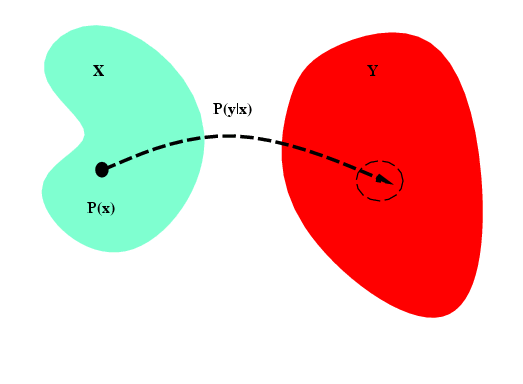
\includegraphics[width=0.7\textwidth]{images/mapping_proba.png}
		\caption{Mapping between the set $\mathcal{X}$ and $\mathcal{Y}$.}
		\label{fig:mapping_proba}
	\end{figure}

	We are trying to estimate the probability $p(Y|X)$ assuming that $X$ and $Y$ share a joint distribution (like described in figure \ref{fig:mapping_proba}).

\newpage

\paragraph{Minimization of the risk :}
	The model which is minimizing the regularized empirical risk, can be found by solving the following optimization problem :
	$$\theta^*=argmin_\theta\sum_{i=1}^n l(y_i,f_\theta(x_i)) + \lambda\Omega(\theta)$$
	Where :
	\begin{itemize}
		\item $l(y_i,f_\theta(x_i))$ is the loss function between the true label $y_i$ and the predicted one $f_\theta(x_i)$
		\item $\lambda\Omega(\theta)$ is the regularization parameter to prevent from over-fitting.
	\end{itemize}

\section{Evaluation}
	The model built will be evaluated by computing the \textbf{log-loss} on predicted probabilities during a \textbf{5-fold cross validation}.

	\subsection{Logistic loss}
		The log-loss measures the accuracy of a classifier. We use it when the model outputs a probability for each class, rather than just the most likely class. That is basically what we aim to do by predicting a probability of defaulting that estimates this precise risk.\\

		The log-loss is a measurement of accuracy that incorporates the idea of probabilistic confidence. It is intimately tied to information theory : log-loss is the cross entropy between the distribution of the true labels and the predictions. Intuitively speaking, entropy measures the unpredictability of something. Cross entropy incorporate the entropy of the true distribution, plus the extra unpredictability when we assume a different distribution than the true distribution. So log-loss is an information-theoretic measure to gauge the ``extra noise'' that comes from using a predictor as opposed to the true labels. The use of log on the error provides extreme punishments for being both confident and wrong. In the worst possible case, a single prediction that something is definitely true when it is actually false will add infinite to your error score and make every other entry pointless. By minimizing the cross entropy, we maximizes the accuracy of the classifier. The mathematical definition of the log-loss is visible below :
		$$L = -\frac{1}{n}\sum_{i=1}^{n}[y_i\log(p_i)+(1-y_i)\log(1-p_i)]$$

	\subsection{5-fold cross validation}
		The model built will be evaluated with a 5-fold cross validation. The entire dataset is split into 5 subsamples and each subsample is used once to validate the model and four times to train it. In figure \ref{fig:5_fold_cv} you can see how each subsample of the whole dataset is used in each fold.

	\begin{figure}[h]
		\centering
		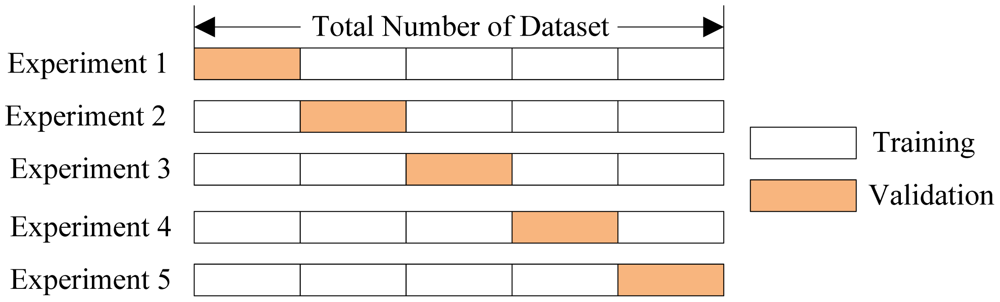
\includegraphics[width=\textwidth]{images/5_fold_cv.png}
		\caption{Each subsample is used once for validation and four times for training.}
		\label{fig:5_fold_cv}
	\end{figure}

	In each fold, one borrower must be either in the training set or the testing set but never in both, to prevent from over fitting (see section \ref{sec:data} for further informations on the data). Here is what is done in each fold (also visible in figure \ref{fig:cv_process}):
	\begin{enumerate}
		\item Build a classifier on a training set
		\item Predict the probabilities of each label on a validation set
		\item Compute the logistic loss
		\item Compute the area under the Receiver Operating Characteristic curve (ROC-AUC score)
	\end{enumerate}

	\begin{figure}[h]
		\centering
		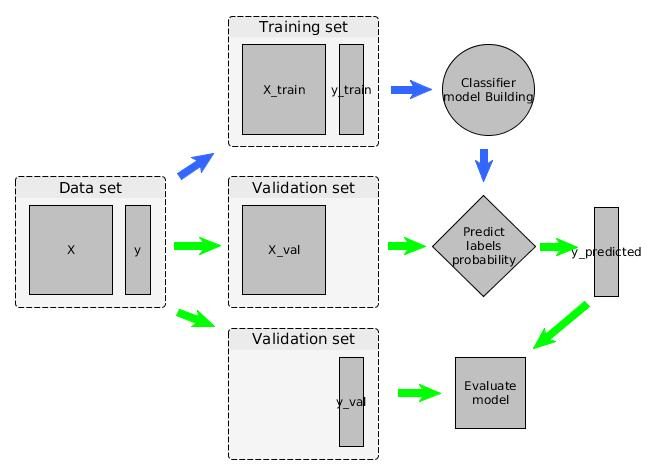
\includegraphics[width=\textwidth]{images/cv_process.jpg}
		\caption{What is done during one fold of cross validation.}
		\label{fig:cv_process}
	\end{figure}

	\subsection{Area Under the Receiver Operating Characteristic Curve (AUC-ROC)}
		To evaluate the model built, we also compute the area under the Receiver Operating Characteristic curve.
		À développer!

\section{Data}\label{sec:data}
	The dataset we are using is provided by the Bitbond lending platform. For confidentiality reasons, the data are anonymized. The dataset contains 2177 loans described by : a loan status, a loan term in months, a loan purpose from a given set, a free text project description, a loan amount, a currency (Bitcoin or USD), the number of rates to pay and those already paid, the publishing and funding time of the loan, a borrower ID, the borrower's employment, the borrower's net income in local currency, the borrower's address (latitude and longitude), some information about the social media connection between the borrower and the Bitbond page (only boolean, due to anonymization).\\

	Among those 2177 loans :
	\begin{itemize}
		\item 608 loans have either the status defaulted (49), fully paid back (391), charged off (119) or 90 days late (49)
		\item We consider only those 608 loans to build our classification model (with a proportion of fully paid back label of 65\% against the rest)
		\item There are 521 distinct borrowers whose 446 have an address defined by their latitude and longitude
	\end{itemize}

\chapter{Features and Classification Models}
\section{Feature engineering}
\label{sec:feature_engi}
	The features from Bitbond that we kept for the estimation of the risk are the following :
	\begin{itemize}[font=\footnotesize]
		\item We kept six categorical features which are :
		\begin{itemize}[font=\footnotesize]
			\item the term of the loan that takes five distinct values : 'term\_12\_months', 'term\_36\_months', 'term\_60\_months', 'term\_6\_months' and 'term\_6\_weeks'.
			\item the social media connections between the borrower and the Bitbond page that are booleans : linkedin, facebook, twitter, paypal and ebay.
		\end{itemize}
		\item We kept three numerical features :
		\begin{itemize}
			\item the location of the borrower on Earth ('address\_lat' and 'address\_lng').
			\item the net incomes in cents made by the borrower in a month ('net\_income\_cents').
		\end{itemize}
		\item We kept a textual feature the free text project description that looks like this :\\
		`I need to make some investments but need to complement the capital, this loan will cover the expenses. Just sit back and enjoy the monthly payments.'
		\item We kept a time feature : the date of application of the loan.
	\end{itemize}

	\subsection{Dealing with categorical feature}
		We used the \href{http://scikit-learn.org/stable/modules/generated/sklearn.preprocessing.LabelEncoder.html}{LabelEncoder} from \textit{scikit-learn} to encode the categorical features as follows :
		\usemintedstyle{tango}
		\begin{minted}[bgcolor=white]{python}
>>> from sklearn.preprocessing import LabelEncoder
>>> le = LabelEncoder()
>>> le.fit(["paris", "paris", "tokyo", "amsterdam"])
LabelEncoder()
>>> list(le.classes_)
['amsterdam', 'paris', 'tokyo']
>>> le.transform(["tokyo", "tokyo", "paris"])
array([2, 2, 1]...)
>>> list(le.inverse_transform([2, 2, 1]))
['tokyo', 'tokyo', 'paris']
		\end{minted}

		After transforming the categorical features, we used \href{http://scikit-learn.org/stable/modules/generated/sklearn.preprocessing.OneHotEncoder.html}{OneHotEncoder} from \textit{scikit-learn} to encode the categorical integer features (produced by the \href{http://scikit-learn.org/stable/modules/generated/sklearn.preprocessing.LabelEncoder.html}{LabelEncoder}) into binary features using a one-hot aka one-of-K scheme. This encoding is needed for feeding categorical data to many \textit{scikit-learn} estimators, notably linear models and SVMs with the standard kernels.
		\usemintedstyle{tango}
		\begin{minted}[bgcolor=white]{python}
>>> from sklearn.preprocessing import OneHotEncoder
>>> enc = OneHotEncoder()
>>> enc.fit([[0, 0, 3], [1, 1, 0], [0, 2, 1], [1, 0, 2]])
OneHotEncoder(categorical_features='all', dtype=<... 'float'>,
       handle_unknown='error', n_values='auto', sparse=True)
>>> enc.n_values_
# Maximum number of values per feature
array([2, 3, 4])
>>> enc.transform([[0, 1, 1]]).toarray()
# 2 columns to encode 0 and 1 for 1st feature,
# 3 columns to encode 0, 1 or 2 for 2nd feature
# and 4 columns to encode 0, 1, 2 or 3 for 3rd feature
array([[ 1.,  0.,  0.,  1.,  0.,  0.,  1.,  0.,  0.]])
		\end{minted}

		In the dataset of 608 loans based on the status that we kept ('defaulted', 'fully\_paid', 'charged\_off' or 'late\_90'), the feature term takes only four distinct values ('term\_60\_months' never present). By transforming the feature term we obtain four binary features. By transforming the five social media connection features we obtained per feature two binary new feature. At the end, we obtained a matrix of 608 raws by 14 columns that can be used for classification.

	\subsection{Dealing with numerical feature}
		An other very interesting feature should have been the borrower's net income in local currency. The main issue with that feature was that it is based on the local currency. So using it like this was nonsense, we had to normalize it in order to have an idea of their incomes on a common basis.\\

		A way to tackle this problem was to use two other features provided by Bitbond : the borrower's location (latitude and longitude). Those one can get us additional features on the borrower region like the cost of living or the standard of living thanks to API like Numbeo or Google. We used the Numbeo API to get the ``Average Monthly Disposable Salary'' of each distinct regions present in the dataset. After getting this new information, we used it to divide the borrower's net income in local currency to create a ratio that should be comparable between the borrowers. We called that feature 'salary'.\\

		The main issue with that procedure was that it cost a huge amount of time, moreover the currencies are not all matching between Bitbond and Numbeo. It produced ratio that can be biased and to find them we have to check borrower by borrower their local currency, their region and their location if they gave one. Because sometimes borrowers are living in a region like Namibia, their currency given by Bitbond is the one of Namibia, but the one given by Numbeo is the one of South Africa.\\

		After checking the more we could (or the most we thought of), we added this ratio in our list of features (matrix of 608 raws by 15 columns).

	\subsection{Dealing with textual feature}
		The free text project description could not be used as it is given. We had to do some text processing before doing anything of it. In fact, raw data, sequence of symbols cannot be fed directly to the \textit{scikit-learn}'s algorithms as most of them expect numerical feature vectors with a fixed size rather than the raw text documents with variable length. We describe below the text processing pipeline that we created.

		\paragraph{Tokenization}
			First of all, we had to tokenize the text into token. To do so, we first needed to tokenize the text into list of sentences. Then we had to tokenize the sentences into list of tokens. Hopefully, there is a python library named \href{http://www.nltk.org/}{\textit{Natural Language Toolkit}} that provides several tools to do text processing. Below you can see an example of the tokenization process :
			\begin{minted}[numberblanklines=true,showspaces=false,breaklines=true,bgcolor=white]{python}
>>> project_description = "I need to make some investments but need to complement the capital, this loan will cover the expenses. Just sit back and enjoy the monthly payments"
>>> Tokenizer().tokenize(project_description)
[['I', 'need', 'to', 'make', 'some', 'investments', 'but', 'need', 'to', 'complement', 'the', 'capital', ',', 'this', 'loan', 'will', 'cover', 'the', 'expenses', '.'], ['Just', 'sit', 'back', 'and', 'enjoy', 'the', 'monthly', 'payments']]
			\end{minted}

		\paragraph{Part-of-Speech Tagging}
			After tokenizing, we computed the Part-of-Speech Tagging (that helps for the lemmatization). It means to find for each word of each sentence its grammatical function : verb, noun, adjective, adverb, pronoun, etc. Here is an example :
			\begin{minted}[numberblanklines=true,showspaces=false,breaklines=true,bgcolor=white]{python}
>>> tokenized_sentences = [['I', 'need', 'to', 'make', 'some', 'investments', 'but', 'need', 'to', 'complement', 'the', 'capital', ',', 'this', 'loan', 'will', 'cover', 'the', 'expenses', '.'], ['Just', 'sit', 'back', 'and', 'enjoy', 'the', 'monthly', 'payments']]
>>> Tagger().tag_sentences(tokenized_sentences)
[[('I', 'PRP'), ('need', 'VBP'), ('to', 'TO'), ('make', 'VB'), ('some', 'DT'), ('investments', 'NNS'), ('but', 'CC'), ('need', 'VBP'), ('to', 'TO'), ('complement', 'VB'), ('the', 'DT'), ('capital', 'NN'), (',', ','), ('this', 'DT'), ('loan', 'NN'), ('will', 'MD'), ('cover', 'VB'), ('the', 'DT'), ('expenses', 'NNS'), ('.', '.')], [('Just', 'RB'), ('sit', 'PRP'), ('back', 'RB'), ('and', 'CC'), ('enjoy', 'VBP'), ('the', 'DT'), ('monthly', 'JJ'), ('payments', 'NNS')]]
			\end{minted}

		\paragraph{Lemmatization}
			Now that we had the Part-of-Speech Tagging of each word, we could find the lemma of each one of them. Before doing that, we had to normalize the Part-of-Speech Tagging to limit them to verb, noun, adjective and adverb because the lemmatizer of the \href{http://www.nltk.org/}{\textit{Natural Language Toolkit}} accept only those four tags. Each word that is neither a verb, an adjective nor an adverb are tagged as noun. Why ? Because by just choosing NN  (noun) for every tag, we can achieve 14\% accuracy testing on one-fourth of the treebank corpus. With JJ (adjective) we get only 5\%. Below you can see the result of the PoS Tagging normalization as input of the lemmatizer and the result of the lemmatization :
			\begin{minted}[numberblanklines=true,showspaces=false,breaklines=true,bgcolor=white]{python}
>>> postagged_sentences = [[('I', 'n'), ('need', 'v'), ('to', 'n'), ('make', 'v'), ('some', 'n'), ('investments', 'n'), ('but', 'n'), ('need', 'v'), ('to', 'n'), ('complement', 'v'), ('the', 'n'), ('capital', 'n'), (',', 'n'), ('this', 'n'), ('loan', 'n'), ('will', 'n'), ('cover', 'v'), ('the', 'n'), ('expenses', 'n'), ('.', 'n')],[('Just', 'r'), ('sit', 'n'), ('back', 'r'), ('and', 'n'), ('enjoy', 'v'), ('the', 'n'), ('monthly', 'a'), ('payments', 'n')]]
>>> Lemmatizer().lemmatize(postagged_sentences)
[['I', 'need', 'to', 'make', 'some', 'investment', 'but', 'need', 'to', 'complement', 'the', 'capital', ',', 'this', 'loan', 'will', 'cover', 'the', 'expense', '.'], ['Just', 'sit', 'back', 'and', 'enjoy', 'the', 'monthly', 'payment']]
			\end{minted}
			We lemmatized every text project description to normalize the vocabulary used by the borrower to limit the sparsity of the vocabulary. (Remark : we could also have done some stemming after the lemmatization to reduct again the vocabulary.)

		\paragraph{Remove stopwords \& puntuation, and transform into bag-of-words modeling}
			Lastly, we just removed the stopwords\footnote{Stopwords are common words that generally do not contribute to the meaning of a sentence, at least for the purposes of information retrieval and natural language processing. These are words such as the and a.}, the punctuation (with regular expression) and we used the \href{http://scikit-learn.org/stable/modules/generated/sklearn.feature_extraction.text.CountVectorizer.html}{CountVectorizer} of \textit{scikit-learn} to transform our list of words into the bag-of-words representation. Below is an example of this representation :
			\begin{minted}[numberblanklines=true,showspaces=false,breaklines=true,bgcolor=white]{python}
>>> project_description1 = "I want to borrow bitcoins to finish the construction of my house."
>>> project_description2 = "I intend to borrow bitcoins to build me a new house."
>>> list_of_description = [project_description1, project_description2]
>>> cv = CountVectorizer()
>>> cv.fit(list_of_description)
>>> cv.vocabulary_
{'bitcoins': 0, 'borrow': 1, 'build': 2, 'construction': 3, 'finish': 4, 'house': 5, 'intend': 6, 'me': 7, 'my': 8, 'new': 9, 'of': 10, 'the': 11, 'to': 12, 'want': 13}
>>> cv.transform(list_of_description).todense()
matrix([[1, 1, 0, 1, 1, 1, 0, 0, 1, 0, 1, 1, 2, 1],
        [1, 1, 1, 0, 0, 1, 1, 1, 0, 1, 0, 0, 2, 0]])
			\end{minted}
		We built a project description word matrix by pruning the vocabulary of words such that it only contained words that :
		\begin{itemize}
			\item Have latin characters and are of length 3 or more characters (token\_pattern='[a-zA-Z]{3,}').
			\item Occur in at least 0.2\% of all documents and at most 95\% of all documents (max\_df=0.95, min\_df=0.002).
		\end{itemize}
		Out of these using the 2000 most frequent words.\\

		The project description word frequency matrix (or bag-of-words representation) is a 2D array where rows represent project descriptions and columns represent words and each cell counts how many times the specific word appears in a given project description. Now that we had the text project description into the bag-of-words representation, we could use it as input of a latent Dirichlet allocation (LDA) model to discover the topics prevalent in the project description collection, and assign topics to the project descriptions.

		\paragraph{Latent Dirichlet Allocation}
			An LDA model describes each topic in terms of a distribution over words, and each project description as a distribution over topics. The problem setting is unsupervised in the sense that only the text in the project descriptions is observed, and all other variables are latent and need to be inferred by the model.
			LDA is a bag-of-words model, meaning that the probabilistic process for a project description does not take into account the order in which the words appear in a project description. This means that for performing inference with the LDA model, it suffices to know which words appear in a project description and how often each word appears. Therefore we will pass the bag-of-words representation of the project descriptions as input.\\

			Using \href{http://scikit-learn.org/stable/modules/generated/sklearn.decomposition.LatentDirichletAllocation.html}{LatentDirichletAllocation} from \textit{scikit-learn}, we trained a LDA model with $K=20$ topics on the project descriptions collection using the project description word frequency matrix (or bag-of-words representation). The new matrix produced by this model has size 608 loans by 20 the probability of each topics in each project description.\\

			To use this new matrix as well as the one of the categorical features, we just concatenate them : it results a 608 by 35 matrix.


	\subsection{Dealing with time feature}
		In order to keep some context in our dataset, we used the date of publication of the loan (published\_at feature). This date is a string formatted as following :
		\begin{minted}[numberblanklines=true,showspaces=false,breaklines=true,bgcolor=white]{python}
'2013-06-21 15:24:55 +0200'
		\end{minted}
		The date could not be used like this. The idea was to convert it in term of number of days past since the earliest date in time of publication of a loan. To do so we first had to extract each string representing the date and to convert it to datetime format. Then we just had to subtract each date to the earliest one in time and to convert that difference in term of the number of day.
		\paragraph{Convert the date time into datetime format}
			Hopefully for us, pandas proposes some methods and functions to do this conversion :
		\begin{minted}[numberblanklines=true,showspaces=false,breaklines=true,bgcolor=white]{python}
>>> published_date = data['published_at']
# First we have to split the string to drop the 3rd part
>>> splited_date = published_date.str.rsplit(' ', expand=True, n=1)
>>> splited_date.ix[0]
0    2013-06-21 15:24:55
1                  +0200
Name: 0, dtype: object
# Then we drop the 2nd column that contains the third part
>>> new_date = published_date.drop(1, axis=1)
>>> new_date.ix[0]
0    2013-06-21 15:24:55
Name: 0, dtype: object
>>> datetime_published = to_datetime(published_date[0], format='\%Y-\%m-\%d \%H:\%M:\%S')
>>> datetime_published.ix[0]
Timestamp('2013-06-21 15:24:55')
		\end{minted}

		\paragraph{Extract the earliest date in time and subtract it to the other}
		Now that our feature date of publication was of type \textit{pandas.tslib.Timestamp}, we could extract the earliest date in time, subtract it to all other date of publication and transform the resulting date into the number day as following :
		\begin{minted}[numberblanklines=true,showspaces=false,breaklines=true,bgcolor=white]{python}
# Extraction of the earliest date in time
>>> first_date = published_date.first.im_self[0]
>>> first_date
Timestamp('2013-06-21 15:24:55')
# Subtracting the date and get the result in a month number basis
>>> data['time_since_published'] = (published_date - first_date).dt.days
		\end{minted}
		We could now use it like this as an indicator of context for the classification. In fact, maybe in a period of economic crisis people may intend to be less honest and default more than in prosperity time.\\

		To use this new feature, we just concatenate it to the previous matrix of categorical features and LDA features : it results a 608 by 36 matrix.


	\subsection{The other features provided by Bitbond}
		We were curious to see if there was a link between defaulting and the location on earth, but we noticed on figure \ref{fig:loc_def} that there is none. So we decided not to use the location features (latitude and longitude).\\

		Concerning the other features, they do not bring any improvement in the classification, except the number of rates already paid. The improvement makes sense but using it not, because it is like using the status as a feature since when a borrower did not paid back it will take each time the value zero. The funding time of the loan is also not usable since at the application time we do not have it.\\

		\begin{figure}[h]
			\centering
			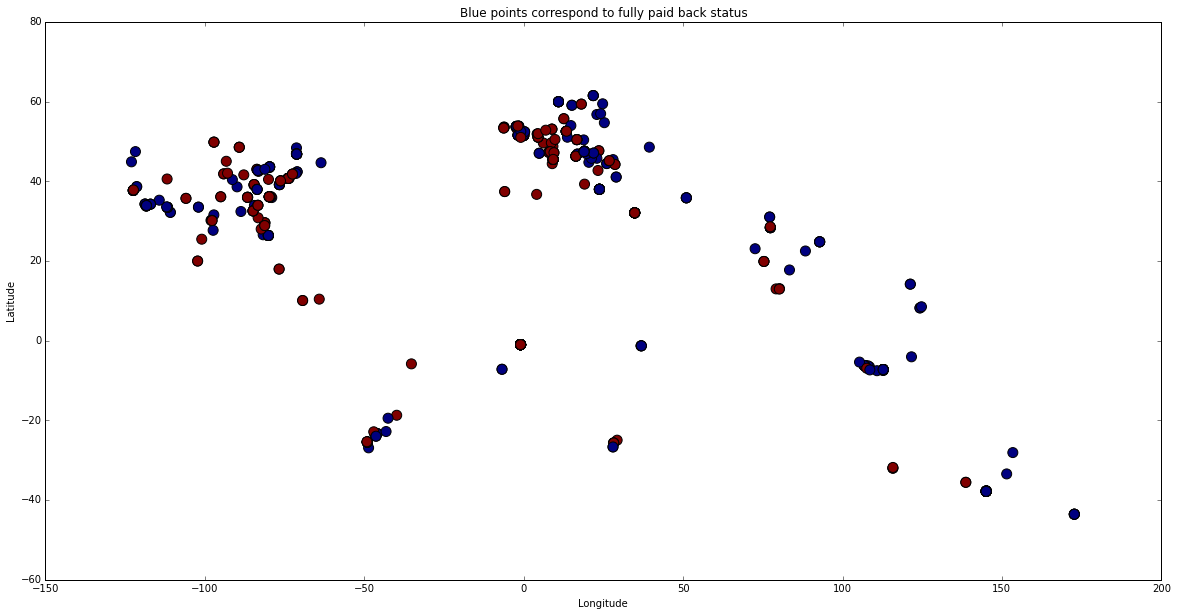
\includegraphics[width=\textwidth]{images/loc_def.png}
			\caption{In red we can see the borrower's location that actually defaulted and in blue paid back.}
			\label{fig:loc_def}
		\end{figure}

\section{Classification models}
\label{sec:models}
	We have to build a model that maps the space of loans to the space of predictions : $$f_\theta:\mathcal{X}\rightarrow \mathcal{Y}$$

	We are doing probabilistic classification. The most obvious model to use, is the Logistic Regression. \textit{scikit-learn} also provides SVMs that can produce probabilities. Those are the two models that we used.

	\subsection{Logistic Regression}
		First a short reminder on the Logistic Regression, here is a quote from \href{http://scikit-learn.org/stable/modules/linear_model.html#logistic-regression}{scikit-learn} about logistic regression :\\

		Logistic regression, despite its name, is a linear model for classification rather than regression. Logistic regression is also known in the literature as logit regression, maximum-entropy classification (MaxEnt) or the log-linear classifier. In this model, the probabilities describing the possible outcomes of a single trial are modeled using a logistic function.\\

		As an optimization problem, binary class L2 penalized logistic regression minimizes the following cost function:
		$$\underset{w,c}{min}\frac{1}{2}w^\intercal w+C\sum_{i=1}^{n}\log{(\exp{(-y_i(X^\intercal_{i} w+c))}+1)}.$$
	\subsection{Support Vector Machine}
	\label{ssec:svm}
		A short reminder on the SVM, here is a quote from \href{http://scikit-learn.org/stable/modules/svm.html}{scikit-learn} about SVM :\\

		A support vector machine constructs a hyper-plane or set of hyper-planes in a high or infinite dimensional space, which can be used for classification. Intuitively, a good separation is achieved by the hyper-plane that has the largest distance to the nearest training data points of any class (so-called functional margin), since in general the larger the margin the lower the generalization error of the classifier.
		\begin{figure}[h]
			\centering
			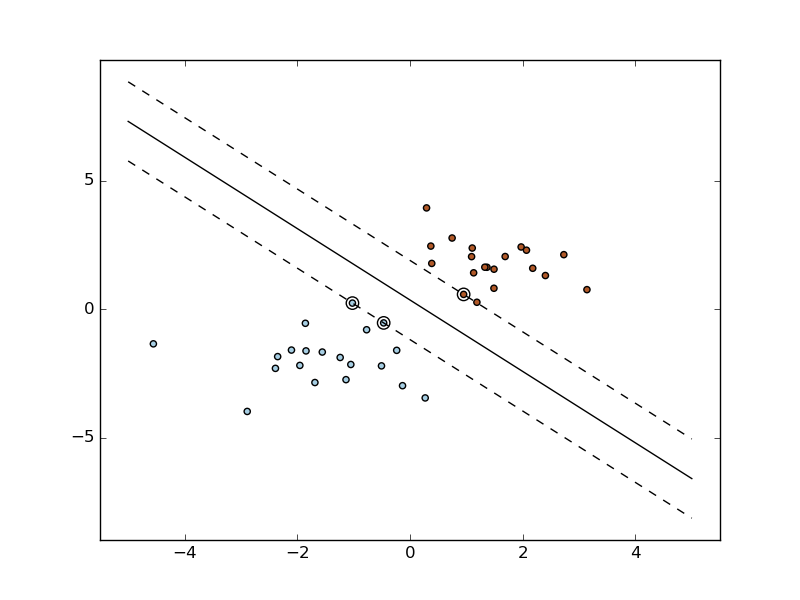
\includegraphics[width=\textwidth]{images/hyperplane.png}
			\label{fig:hyperplane}
		\end{figure}

		Given training vectors $x_i \in \mathbb{R}^p$, $i=1,..., n$, in two classes, and a vector $y \in \{1, -1\}^n$, SVC solves the following primal problem :
		\begin{equation*}
			\begin{aligned}
				& \underset{w,b,\zeta}{min}
				& & \frac{1}{2}w^\intercal w+C\sum_{i=1}^{n}\zeta_i \\
				& subject~to
				& & y_i(w^\intercal \phi(x_i)+b) \geq 1-\zeta_i\\
				& & & \zeta_i \geq 0,i=1,\ldots,n
			\end{aligned}
		\end{equation*}

		When the constructor option probability is set to True, class membership probability estimates (from the methods predict\_proba and predict\_log\_proba) are enabled. In the binary case, the probabilities are calibrated using Platt scaling: logistic regression on the SVM’s scores, fit by an additional cross-validation on the training data.\\

		Needless to say, the five-fold cross-validation involved in Platt scaling is an expensive operation for large datasets.\\

		For the classification task we built a \href{http://scikit-learn.org/stable/modules/generated/sklearn.linear_model.LogisticRegression.html#sklearn.linear_model.LogisticRegression}{Logistic Regression} model and a \href{http://scikit-learn.org/stable/modules/generated/sklearn.svm.SVC.html#sklearn.svm.SVC}{SVC} model with those parameters :
		\begin{minted}[bgcolor=white]{python}
logic_reg = LogisticRegression()
svc = SVC(kernel='linear', probability=True)
		\end{minted}
		Remark : The Logistic regression model is based on the same library (liblinear) as SVC model.

	\subsection{Matrix dimensionality reduction}
		Because the computation of the probabilities by the SVM is very slow (due to internal five-fold cross validation), we used dimensionality reduction model to reduce the dimension of the input matrix. We tried several models and especially : (kernel) Principal Component Analysis, t-SNE and Linear Discriminant Analysis.\\

		In figures \ref{fig:kpca}, \ref{fig:tsne} and \ref{fig:lda} are respectively visible the result of kernel PCA (with rbf kernel), of t-SNE and of LDA with two components.\\

		\begin{figure}[h]
			\centering
			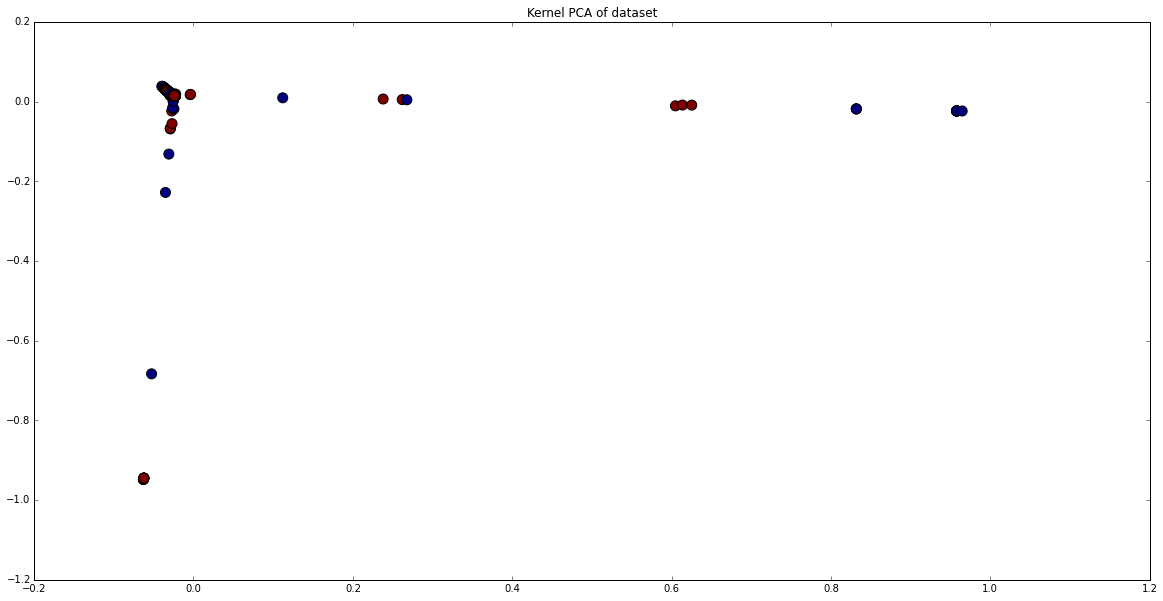
\includegraphics[width=0.9\textwidth]{images/kpca.png}
			\caption{Dimensionality reduction : kernel PCA (rbf kernel) with two components.}
			\label{fig:kpca}
		\end{figure}
		\begin{figure}[h]
			\centering
			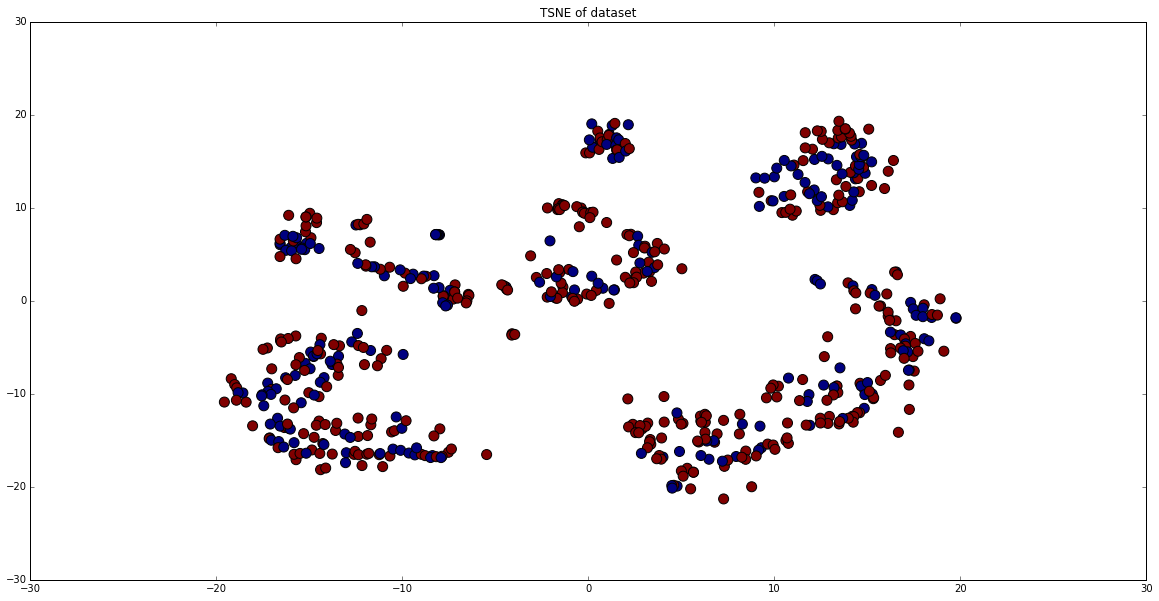
\includegraphics[width=0.9\textwidth]{images/tsne.png}
			\caption{Dimensionality reduction : t-SNE with two components.}
			\label{fig:tsne}
		\end{figure}
		\begin{figure}[h]
			\centering
			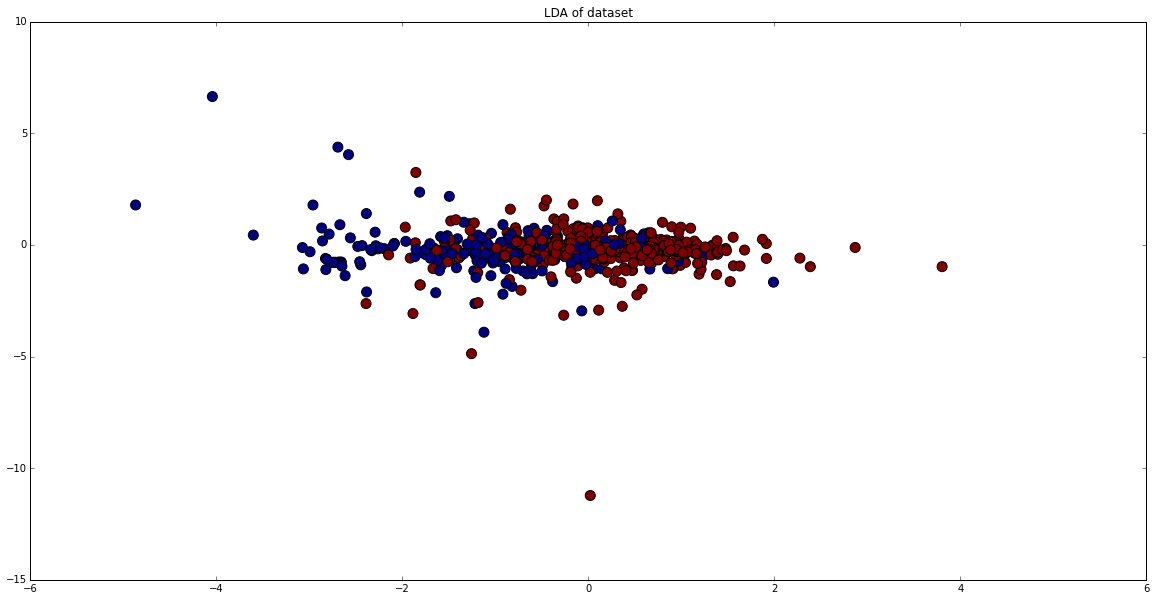
\includegraphics[width=0.9\textwidth]{images/lda.png}
			\caption{Dimensionality reduction : Linear Discriminant Analysis with two components.}
			\label{fig:lda}
		\end{figure}
		We can say that the results of kernel PCA and t-SNE with two components are not as good as the result of LDA which outputs the data points of each labels not mixed up. The input data of those models are the matrix produced after the feature engineering work done in the last part : a matrix of size $(608,36)$.\\

		For each model, we tried more than two components (the number of components for dimensionality reduction) and also other kernel (for kernel PCA), but the results makes the next task (the estimation of the risk) producing worse log loss results. Moreover the first two components of the kernel PCA explained variance 98.9\% of the variance.

\chapter{Evaluation}
\section{Performances of the Logistic Regression}
	In this section, when we describe the effect of each feature on the estimation of the risk of defaulting, we are dealing with the features specified in section \ref{sec:feature_engi}.\\

	By using all the features we considered in section \ref{sec:feature_engi}, we obtained an average log loss on the five folds of 0.66. Let's see the influence of each feature.

	\subsection{Impact of the 'salary' feature}
		This is our only numerical feature and we were very surprised to notice that it make a very big difference in the estimation of the risk but not in the good way. In fact, without it the average log loss on the five folds drops from 0.66 to 0.56. So we rejected it (also for the rest of the evaluation section).

	\subsection{Impact of the latent features}
		The latent features produced by the Latent Dirichlet Allocation based on the textual project description make the area under the ROC curve improves. But we observed thanks to the area under the ROC curve that even if the area is better, the classifier becomes less robust. In fact we noticed on the area under the ROC curve that the classifiers built during the cross validation had an area under the ROC curve less similar and close, and more irregular.
		On top of that, the average log loss on the five folds drop from 0.56 to 0.55 without them, so 1\% better. This goes in the same way as the irregularity of the area under the ROC curve.\\

		We took the decision to throw them away (also for the rest of the evaluation section) because even if the area under the ROC curve is better, that does not correspond to our problem setting which consist to estimate the risk of default. You can see in figure \ref{fig:auc_latent} the area under the ROC curve with and without the latent features.
		\begin{figure}[h!]
            \centering
            \begin{subfigure}[b]{0.98\textwidth}
                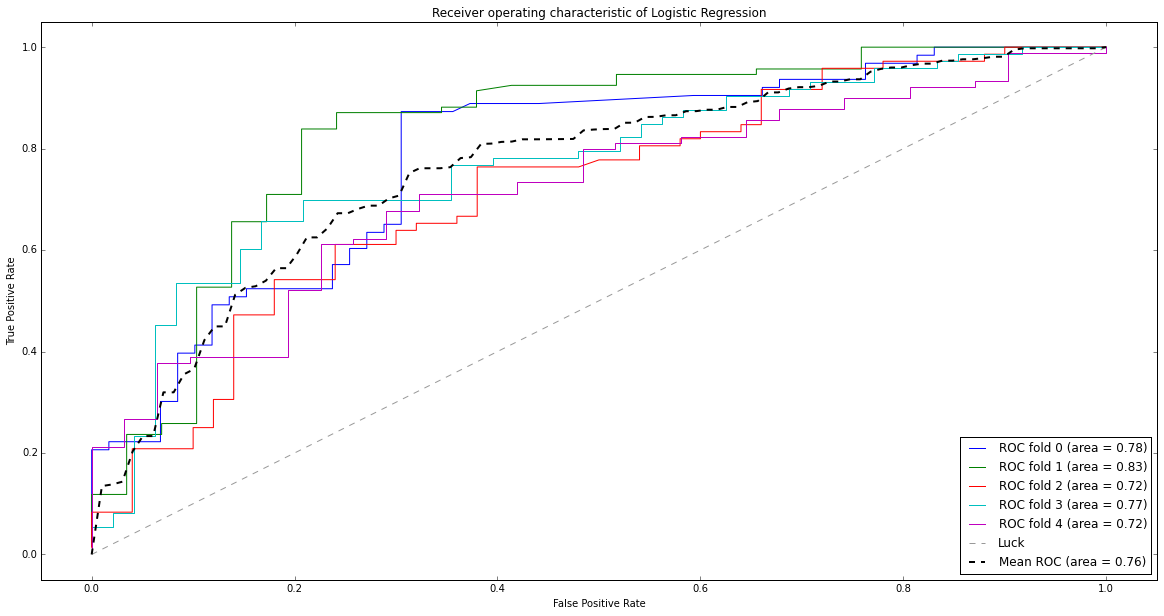
\includegraphics[width=\textwidth]{images/auc_without_latent.png}
                \caption{area under the ROC curve without the latent features.}
                \label{fig:auc_without_latent}
            \end{subfigure}
            \begin{subfigure}[b]{0.98\textwidth}
                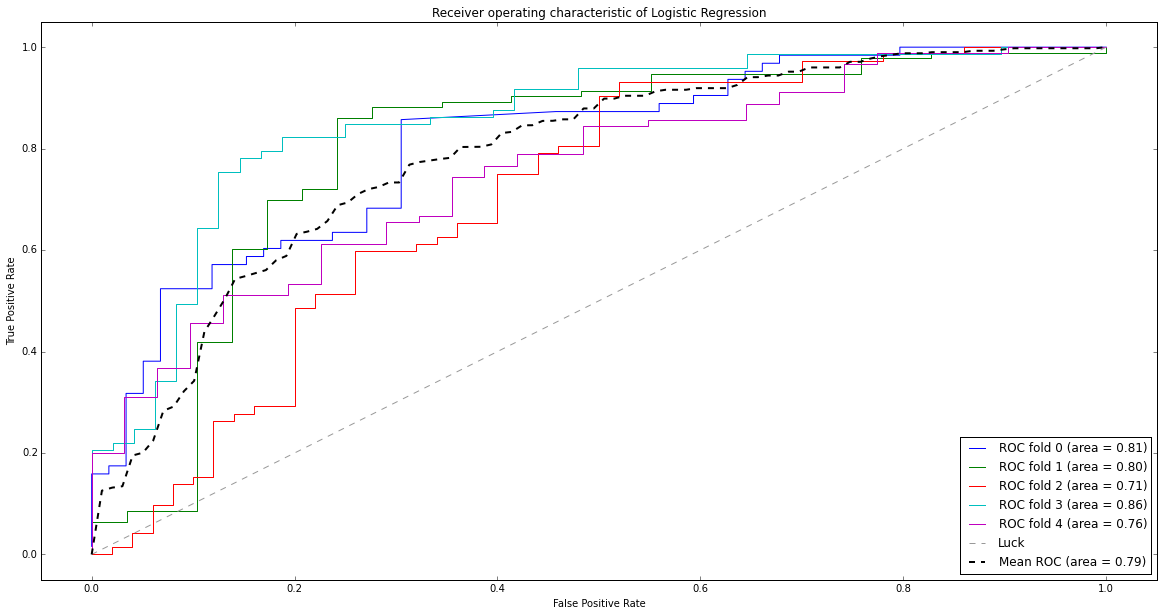
\includegraphics[width=\textwidth]{images/auc_with_latent.png}
                \caption{area under the ROC curve with the latent features.}
                \label{fig:auc_with_latent}
            \end{subfigure}
            \caption{Difference of area under the ROC curve with or without the latent features.}
            \label{fig:auc_latent}
        \end{figure}

	\subsection{Impact of the time feature}
		The time feature built based on the publication date of the loan really help the classifier. In fact the log loss increase from 0.55 to 0.59 without it. We explain that with the idea of context. In fact the contextual information brought by this feature informs of the economic situation and helps the estimation of the risk which is related to the economic situation. There may be more defaulting in certain periods of time than others.\\

		This kind of lending platform, like Bitbond, were born with the arrival of the currency Bitcoin. Moreover this currency were very popular during the Greek crisis for instance when all bank were closed. The popularity aspect implies an more important use of those platforms and if there are more use there is a higher probability of defaulting among the borrowers.\\

		This feature is kept for the estimation of the risk.

	\subsection{Impact of the Linear Discriminant Analysis}
		The Linear Discriminant Analysis done to reduce the dataset dimension before building the logistic regression model, has no impact on the log loss computation which is obviously normal since it is a linear model like the logistic regression. The only utility is when we build a SVM model that compute probability for each class, because the probability computation includes a five folds cross validation (for more detail see subsection \ref{ssec:svm}).

\section{Performances of the SVM}
	The performances of the SVM are basically the same. This due to the fact that both model are based on the same library (liblinear). We obtain like with logistic regression model a log loss of 0.55 with the same features and with or without the Linear Discriminant Analysis. This last one just makes the computation of the model faster : 2 minutes and 30 seconds without it and 3 seconds with.

\section{Hyperparameter setting}
	To set the hyperparameter we tried to use the \href{http://scikit-learn.org/stable/modules/generated/sklearn.grid_search.GridSearchCV.html#sklearn.grid_search.GridSearchCV}{GridSearchCV} of \textit{scikit-learn}. But after six hours it was still not done. That is why we chose to set it manually by trying different values for the C parameter of the \href{http://scikit-learn.org/stable/modules/generated/sklearn.linear_model.LogisticRegression.html#sklearn.linear_model.LogisticRegression}{LogisticRegression} by doing a nested five folds cross validation. We came to the conclusion that a $C=1$ was the best choice.

\chapter{Conclusion}
To conclude, the main difficulties to handle concerns the feature engineering and especially the different currencies. In fact it is very hard to normalize the incomes of the borrower on a common basis. Maybe a solution would be to fix a threshold and transform the incomes into a categorical feature. Moreover, identifying the outliers among the borrowers is also not obvious at all, since there is no real criterion to use.\\

Categorical features stay easier to use than numerical ones because there is no normalization to do like with numerical one.\\

Including a temporal feature like we did by using the date of publication of the loan is helping very nicely the estimation of the risk of default, thanks to the inclusion of some contextual information into the dataset.\\

Some improvement tracks could be the following :
\begin{itemize}
	\item Use the lending club data to get some additional data on the loans and the borrowers.
	\item Model the loan borrow as a Markov model (with a 6 months period for instance) and in each step of the Markov process evaluate the risk.
\end{itemize}

% Bibliographie
%\bibliographystyle{plain}
\printbibliography

% Annexes
\clearpage
\appendix
\chapter{Annexes}
\input{parties/06-Annexe.tex}

\end{document}
